Das OSI-Modell besteht aus sieben Schichten und ist eine allgemeine Beschreibung
bzw. Designrichtlinie f{\"u}r Kommunikationsprotokolle (siehe Abb.
\ref{fig:OSI_M}).

\begin{figure}[H]
\centering
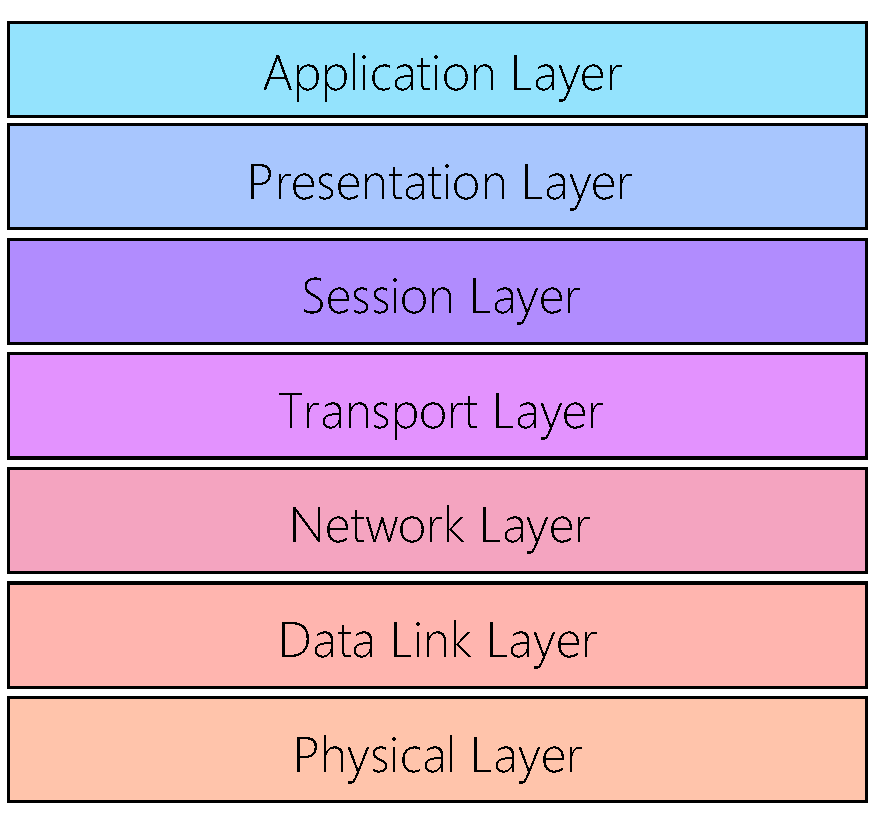
\includegraphics[scale=.3]{OSI_M.pdf}
\caption{Das OSI-Referenzmodell}
\label{fig:OSI_M}
\end{figure}

\textbf{Physical Layer}

Der Physical Layer stellt eine physische Verbindung {\"u}ber das jeweilige
Medium her (z.B. Kupferkabel, Wireless etc.). Hier findet die eigentliche
Bit{\"u}bertragung statt.

\textbf{Data Link Layer}

Der Data Link Layer soll eine sichere {\"U}bertragung gew{\"a}hrleisten. Diesem
obliegt somit das Herstellen einer Ende-zu-Ende Verbindung (Link) um eine
{\"U}bertragung zu erm{\"o}glichen. Dazu geh{\"o}rt die Einteilung der Daten in
Frames, das hinzuf{\"u}gen von Pr{\"u}fsummen sowie die Kanalkodierung und eine
Datenflusskontrolle (Protokollbeispiele: Ethernet, FDDI).

\textbf{Network Layer}

Der Network Layer sorgt f{\"u}r die Weitervermittlung von Datenpaketen. Diesem
obliegt die Adressierung von Datenpaketen (via IP) und das Routing (Aufbau von
Routingtabellen etc.). Protokollbeispiele in dieser Schicht: IP, ICMP.

\textbf{Transport Layer}

Die Aufgaben des Transport Layer sind die Segmentierung des Datenstroms sowie
Stauvermeidung und Bereitstellung von Felersicherungs- und
Fehlerbehebungsverfahren (Protokollbeispiele: TCP, UDP).

\textbf{Session Layer}

Zu den Aufgaben des Session Layer geh{\"o}ren die Handhabung von
Verbindungsabbr{\"u}chen und das daraus resultierende Setzen von
Sicherungspunkten (Checkpoints). Diese erm{\"o}glichen eine Wiederaufnahme
nach einem erfolgten Abbruch. Somit wird eine st{\"a}ndige synchronit{\"a}t der
Dienste gew{\"a}rleistet (Protokollbeispiele: HTTP, FTP).

\textbf{Presentation Layer}

Der Presentation Layer erm{\"o}glicht eine Darstellung von Daten in
einer unabh{\"a}ngigen Form (dies garantiert einen Datenaustausch zwischen
unterschiedlichen Systemen). Desweiteren werden die Daten hier komprimiert und
verschl{\"u}sselt (Protokollbeispiele: HTTP, FTP).

\textbf{Application Layer}

Der Application Layer verwaltet den Zugriff der Anwendung auf das Netzwerk
(Protokollbeispiele: HTTP, FTP).
